
\section{Experiments}

\begin{table}[t]
\centering
%\footnotesize
\scriptsize
\caption{\textbf{Evaluation of different methods on GSM8K and COQA.} The best result (excluding origin) in each column is highlighted in bold. Comp* refers to the theoretical time complexity for each method to select critical KV cache tokens, where $\mathcal{O}(1)$ denotes constant time complexity, and $T$ represents the theoretical computation time for a dense attention mechanism.}
\label{tab:gsm_coqa}
\begin{tabular}{l|l|cccccc}
\toprule
Model & Method & $\hat{\rho}$ & GSM8K $\uparrow$ & COQA $\uparrow$ & Comp* $\downarrow$ \\
\midrule
\multirow{12}{*}{\shortstack{LLaMA2\\-7b-chat}}
& Original  & -  & 0.2297/0.2297 & 0.5997 & - \\
& H2O \cite{zhang2023h2o}   & -        & 0.0986/0.0144 & 0.4952 & $\mathcal{O}(1)$ \\
& Quest \cite{tang2406quest}  & -       & 0.0478/0.0462 & 0.5713 & 0.1250$T$ \\
& DS \cite{yang2024post}  & -   & 0.1713/0.1706 & 0.5978 & 0.0625$T$ \\
\cmidrule{2-6}
& Hshare-1 \cite{wuhshare} & 0.281  & 0.1803/0.1703 & 0.5898 & 0.0180$T$ \\
& Hshare-2 \cite{wuhshare} & 0.125   & 0.1524/0.1145 & 0.5672 & 0.0080$T$ \\
\cmidrule{2-6}
& \multirow{3}{*}{CIS (ours)}  & 0.164  & \textbf{0.1842}/\textbf{0.1827} & 0.6085 & 0.0104$T$ \\
&  & 0.087   & 0.1804/0.1782 & 0.6072 & 0.0055$T$ \\
&  & \textbf{0.062}   & 0.1759/0.1751 & 0.6068 & \textbf{0.0039}$T$ \\
\cmidrule{2-6}
& \multirow{3}{*}{CIS$^\ast$ (ours)}  & 0.161  & 0.1812/0.1804 & \textbf{0.6063} & 0.0103$T$ \\
&  & 0.084   & 0.1789/0.1782 & 0.6063 & 0.0047$T$ \\
&  & 0.063   & 0.1736/0.1729 & 0.6083 & 0.0040$T$ \\
\midrule
\multirow{10}{*}{\shortstack{LLaMA3\\-70b}} 
& Original  & -   & 0.8067/0.8052 & 0.7085 & - \\
& DS \cite{yang2024post}   & - & 0.7415/0.7392 & 0.7045 & 0.0625$T$ \\
\cmidrule{2-6}
& Hshare-1 \cite{wuhshare} & 0.281  & 0.7512/0.7437 & 0.7010 & 0.0180$T$ \\
& Hshare-2 \cite{wuhshare} & 0.125   & 0.7415/0.7346 & 0.6960 & 0.0080$T$ \\
\cmidrule{2-6}
& \multirow{3}{*}{CIS (ours)}  & 0.183  & \textbf{0.7613/0.7592} & 0.7045 & 0.0117$T$ \\
&  & 0.082   & 0.7553/0.7526 & 0.7021 & 0.0052$T$ \\
&  & 0.064   & 0.7528/0.7511 & 0.7003 & 0.0041$T$ \\
\cmidrule{2-6}
& \multirow{3}{*}{CIS$^\ast$ (ours)}  & 0.179  & 0.7584/0.7556 & \textbf{0.7068} & 0.0114$T$ \\
&  & 0.079   & 0.7542/0.7527 & 0.7003 & 0.0050$T$ \\
&  & \textbf{0.061}   & 0.7536/0.7504 & 0.7001 & \textbf{0.0038}$T$ \\
\midrule
\multirow{10}{*}{\shortstack{Mistral\\-7b}} 
& Original & -   & 0.3821/0.3813 & 0.6758 & - \\
& DS \cite{yang2024post} & -  & 0.3262/0.3227 & 0.6693 & 0.0625$T$ \\
\cmidrule{2-6}
& Hshare-1 \cite{wuhshare} & 0.281   & 0.3199/0.3154 & 0.6560 & 0.0180$T$ \\
& Hshare-2 \cite{wuhshare} & 0.125   & 0.2818/0.2684 & 0.6387 & 0.0080$T$ \\
\cmidrule{2-6}
& \multirow{3}{*}{CIS (ours)} & 0.194  & \textbf{0.3325/0.3302} & 0.6703 & 0.0124$T$ \\
&  & 0.088   & 0.3281/0.3275 & 0.6684 & 0.0056$T$ \\
&  & \textbf{0.065}   & 0.3233/0.3201 & 0.6710 & \textbf{0.0041}$T$ \\
\cmidrule{2-6}
& \multirow{3}{*}{CIS$^\ast$ (ours)} & 0.189  & 0.3292/0.3257 & 0.6691 & 0.0121$T$ \\
&  & 0.091   & 0.3216/0.3204 & 0.6714 & 0.0058$T$ \\
&  & 0.068   & 0.3204/0.3175 & \textbf{0.6754} & 0.0043$T$ \\
\bottomrule
\end{tabular}
\end{table}


\subsection{Experimental Setup}

We evaluate our CPE on two widely-used model families: LLaMA~\cite{touvron2023llama} and Mistral~\cite{jiang2023mistral7b}. Specifically, we select LLaMA2-7B-Chat, LLaMA3-70B, and Mistral-7B for our experiments. As baselines, we select one TDO method H2O~\cite{zhang2023h2o}, two QAA algorithms: Quest~\cite{tang2406quest} and DS~\cite{yang2024post}, as well as a SOTA retrieval-based PoHS instantiation: HShare~\cite{wuhshare}. We report results on GSM8K~\cite{cobbe2021gsm8k}, COQA~\cite{reddy2019coqa}, and LongBench~\cite{bai2023longbench}.


In our CPE, we adopt the following default hyperparameters. For CIS, we set the similarity threshold $\tau\!=\!0.8$, and apply dilation on the $m \!=\! \lfloor k/3\rfloor$ highest-score indices with radius $r=1$. Pruning and freezing of PSAW and ETF start from $\ell_s \!=\! \lfloor 3N/4 \rfloor$ for a model with $N$ layers. PSAW uses $\phi \!=\! 0.7$ and $\alpha \!=\! 1$, while ETF uses $\psi \!=\! 0.5$ and $\gamma \!=\! 1$. 

Because CIS performs head-level KV sharing to avoid full retrieval, we define the \emph{per-step retrieval ratio} $\rho_t\!=\!\frac{R_t}{H\cdot N}$ to measure the retrieval frequency, where $R_t$ is the number of performed head–layer retrieval at step $t$, and $H\cdot N$ is the amount required by a naïve top-$k$ oracle. The ratio $\rho_t$ is controlled by the CIS block size $s$ and the similarity threshold $\tau$. In reports, we present the averaged ratio $\hat{\rho}=\tfrac{1}{T}\sum^{T}\rho_t$ over the $T$ generation steps. 


\subsection{Results on GSM8K and COQA}
\label{sec:gsm8k&coqa}

%\paragraph{Datasets and Metrics}
\subsubsection{Datasets and Metrics}
We perform zero-shot evaluation with LM-Eval on the GSM8K~\cite{cobbe2021gsm8k} and COQA~\cite{reddy2019coqa} benchmarks. GSM8K comprises roughly 8 000 grade-school mathematics problems, whereas COQA targets multi-turn conversational question answering. The mean input lengths are about 500 tokens (GSM8K) and 2 000 tokens (COQA). Following prior work, we report both flexible and strict exact-match (EM) accuracy on GSM8K, and EM on COQA.

%\paragraph{Inference Details}
\subsubsection{Inference Details}
We apply TSA in the decoding stage and solely evaluate CIS as presented in Table~\ref{tab:gsm_coqa}. We select a critical KV budget $C_t \!=\! 128$ ~\cite{wuhshare}. For CIS and Hshare, we set $C_{\text{local}} \!=\! 32$, and $k \!=\! 88$ in the middle. Since CIS dilation incurs additional KV budget during sharing, we therefore additionally include a variant CIS$^\ast$, which sets $k=72$, yielding its average budget close to 128. We choose $s\in\{8,16,20\}$ to vary $\hat{\rho}$.



\begin{table*}[t]

\footnotesize
\centering
\caption{\textbf{Evaluation of different methods on sixteen English datasets in Longbench} and the best result in each row (excluding the original) is highlighted in bold. Here, the retrieval complexity of H2O, Quest, DS, and HShare is just the same with Table~\ref{tab:gsm_coqa}.}
\label{tab:longbench}
\begin{tabular}{lcccc|cc|cc|cc|cc}
\toprule
\multicolumn{1}{c}{\multirow{2}{*}{\textbf{Dataset}}} & \multicolumn{12}{c}{\textbf{Method}} \\
\cmidrule(lr){2-13}
 & Original & H2O \cite{zhang2023h2o} & Quest \cite{tang2406quest} & DS \cite{yang2024post} & \multicolumn{2}{c|}{HShare \cite{wuhshare}}  & \multicolumn{2}{c|}{CIS (ours)} & \multicolumn{2}{c|}{CIS$^\ast$ (ours)} & \multicolumn{2}{c}{CPE (ours)}\\
\midrule

$\hat{\rho}$ & - & - & - & - & 0.281 & 0.125 & 0.177 & 0.083 & 0.164 & 0.085 & 0.174 & 0.079\\

\midrule

MultiNews   & 26.22 & 24.88 & \textbf{26.49} & 26.30 & 26.05 & 25.22 & 26.47 & 25.98 & 26.18 & 26.40 & 26.11 & 26.02\\
Musique            & 8.65  & 6.24  & 4.62 & 8.72  & 8.42  & 8.09 & 8.47 & 6.98 & 8.74 & 8.68 & 8.69 & 7.50\\
HotpotQA  & 27.72 & 27.58 & 21.94 & 27.44 & 27.32 & \textbf{29.13} & 27.54 & 28.64 & 26.72 & 27.60 & 27.39 & 27.10\\
Qasper & 21.88 & 17.32 & 16.96 & 20.98 & 20.12 & 19.60 & 21.24 & 21.18 & 20.87 & 20.79 & 20.94 & \textbf{21.63}\\
2WikiMQA  & 31.18 & 31.38 & 29.42 & 32.01 & 31.46 & 31.43 & \textbf{32.51} & 30.78 & 30.05 & 30.70 & 29.06 & 31.15\\
Repo-P & 52.14 & \textbf{51.81} & 50.24 & 48.44 & 50.79 & 51.63 & 50.99 & 50.03 & 50.65 & 50.88 & 51.64 & 51.12\\
TriviaQA  & 83.09 & 81.90 & 82.42 & 83.23 & \textbf{83.91} & 82.16 & 79.57 & 81.46 & 81.04 & 79.76 & 79.78 & 81.35\\
Trec   & 64.5  & 62.5  & 64.0 & 61.05 & 60.5  & 58.5 & 62.5 & 63.5 & 64.5 & 62.5 & \textbf{65.0} & 62.0\\
Qmsum   & 20.91 & 20.74 & \textbf{21.36} & 20.75 & 20.59 & 20.74 & 20.53 & 20.93 & 20.98 & 20.92 & 20.78 & 20.66\\
NarrativeQA  & 18.83 & 17.01 & \textbf{18.21} & 17.54 & 17.31 & 17.31 & 17.90 & 17.05 & 17.65 & 16.30 & 16.55 & 17.96\\
GovReport   & 26.55 & 23.45 & 25.46 & \textbf{27.04} & 25.85 & 25.85 & 26.63 & 26.39 & 26.07 & 26.39 & 25.63 & 25.78\\
LCC    & 58.26 & 56.55 & \textbf{56.74} & 54.87 & 56.23 & 56.11 & 55.35 & 54.43 & 54.89 & 55.10 & 55.62 & 54.22\\
PC      & 2.77  & 1.87  & 2.33 & 3.15 & 2.30  & 2.30 & 2.69 & 3.12 & 2.38 & \textbf{3.34} & 3.27 & 1.93\\

Samsum  & 41.01 & 40.18 & 40.91 & \textbf{41.30} & 39.77 & 40.02 & 40.96 & 40.52 & 39.04 & 39.68 & 40.11 & 40.19\\
PR-EN & 6.5 & 5.0   & 6.5  & 6.0  & 6.0   & 6.0 & 8.5 & 7.0 & 6.0 & \textbf{9.5} & 6.0 & 6.0\\
MQA-EN    & 36.15 & 33.64 & 31.99 & 35.83 & 34.08 & 32.37 & 36.64 & 36.54 & 37.29 & 37.06 & 37.47 & \textbf{37.96}\\
\midrule
Average   & 32.90 & 31.38 & 31.35 & 32.11 & 31.97 & 31.49 & \textbf{32.40} & 32.15 & 32.06 & 32.22 & 32.11 & 32.02\\
\bottomrule
\end{tabular}
\end{table*}


%------------------------------------------------------
\begin{figure}[!t]
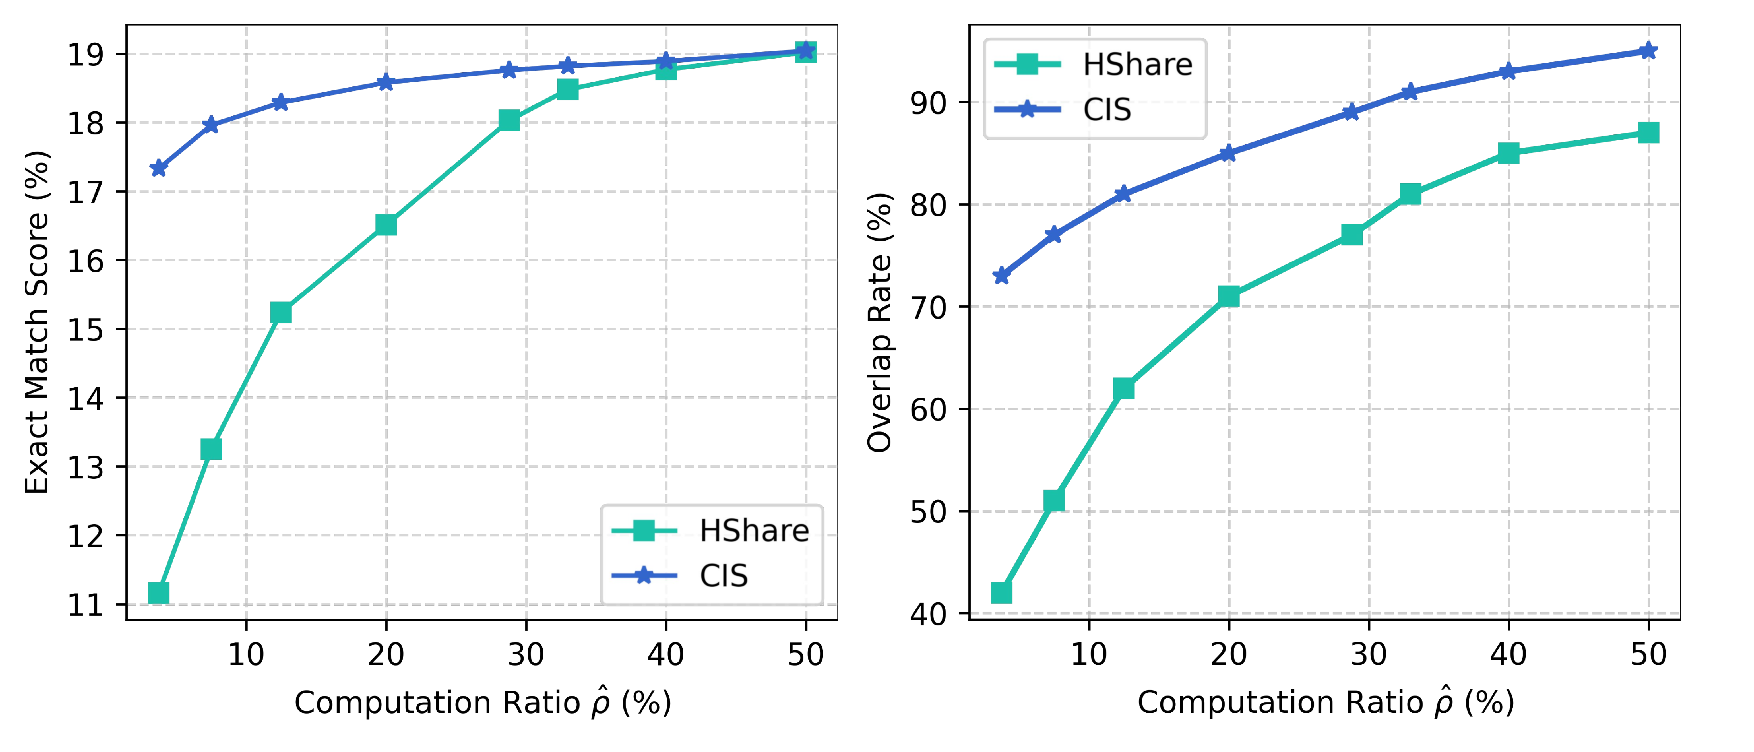
\includegraphics[width=0.48\textwidth]{assets/cis-vs-hshare.pdf}
\centering
\vspace{-1em}
    \caption{\textbf{CIS vs. HShare on GSM8K across computation ratios.} \emph{Left}: Exact-match score accuracy comparisons. \emph{Right}: Overlap comparisons between each method’s retrieved critical set and the top-$k$ oracle.}
    \label{fig:cis_vs_hshare}
    %\vspace{-1.5em}
\end{figure}
%--------

%\paragraph{Result Analysis}
\subsubsection{Result Analysis}


As shown in Table~\ref{tab:gsm_coqa}, CIS and its budget-matched variant CIS$^\ast$ consistently deliver a superior accuracy–efficiency trade-off to PoHS baselines on GSM8K and COQA. On LLaMA-2-7B-Chat, CIS at low selection cost already surpasses SOTA HShare, i.e., $40$–$55\%$ lower complexity at higher accuracy. The advantage widens on LLaMA-3-70B with deeper layers, consistent with reduced cross-layer error accumulation under sharing. CIS$^\ast$ still outperforms HShare at matched budgets, isolating selection \emph{quality} rather than capacity as the driver of the gains. Efficiency is materially better. For instance, on LLaMA-3-70B, CIS uses $0.0052T$ selection cost versus DS’s $0.0625T$.


To further evaluate the accuracy-efficiency trade-offs of CIS, we compare the results of HShare and CIS under different computation ratios on GSM8K. As shown in Fig.~\ref{fig:cis_vs_hshare}(left), when computation ratio is below 30\%, the performance of HShare degrades sharply, while CIS maintains high accuracy. From the perspective of retrained attention mass, Fig.~\ref{fig:cis_vs_hshare}(right) shows that the average overlap of HShare collapses at low computation ratio. These results further demonstrate that the selection quality of CIS is much better than HShare under aggressive sharing.

% As shown in Tab.~\ref{tab:gsm_coqa}, CIS and its budget-matched variant CIS$^\ast$ consistently deliver a superior accuracy–efficiency trade-off to PoHS baselines on GSM8K and COQA. On LLaMA-2-7B-Chat, CIS at low selection cost already surpasses SOTA HShare: CIS attains $0.1842/0.1827$ (flex/strict) with selection cost $0.0104T$, versus HShare(3/4-3/4-1/2) at $0.1803/0.1703$ and $0.0180T$, i.e., $40$–$55\%$ lower complexity at higher accuracy. These gains indicate that CIS under PrHS tightly controls induced error. CIS also shows strong strict–flex robustness on GSM8K (only $0.1842\!\to\!0.1827$ across various computation ratios), whereas HShare drops from $0.1803$ to $0.1703$, suggesting genuine reasoning accuracy rather than formatting artifacts. The advantage widens on LLaMA-3-70B with deeper layers, consistent with reduced cross-layer error accumulation under sharing.

% CIS$^\ast$ still outperforms HShare at matched budgets, isolating selection \emph{quality} rather than capacity as the driver of the gains. Efficiency is materially better: on LLaMA-3-70B, CIS uses $0.0052T$ selection cost versus DS’s $0.0625T$, and across settings CIS operates at $0.0041$–$0.0117T$ compared to HShare’s $0.0180T$, sharpening the accuracy–efficiency frontier. Even under extreme sharing ($\hat{\rho}\!\approx\!0.06$–$0.08$), CIS remains competitive. On COQA, CIS and CIS$^\ast$ are near-dense or better—$0.6103$ on LLaMA-2-7B-Chat exceeds dense $0.5997$, and $0.7068$ on LLaMA-3-70B is close to $0.7085$—indicating that conversational understanding is well preserved.

% To further evaluate the accuracy-efficiency trade-offs of CIS, we compare the results of HShare and CIS under different computation ratios on GSM8K. Fig.~\ref{fig:cis_vs_hshare}(left) plots the EM-computation curve. When computation ratio is high, the accuracy gap between CIS and HShare~\cite{wuhshare} remains relatively small. Below 30\%, the performance of HShare degrades sharply, while CIS maintains high accuracy. From the perspective of retrained attention mass, Fig.~\ref{fig:cis_vs_hshare}(right) shows the average overlap of the true positive of retrieved critical set compared to top-k oracle. Similar to EM, HShare’s overlap rate collapses at low computation ratio. Inspection reveals that HShare's coarse sharing schedules propagate indices between queries with low semantic similarity. Moreover, even for heads with high semantic similarity, its shared set is fragmented (Fig.~\ref{fig:index-frag}), missing many true positives. These problems drastically reduces its recall. CIS, by contrast, maintains a much higher overlap rate even under aggressive sharing.


\subsection{Longbench}
\label{sec:longbench}

%\paragraph{Datasets and Metrics}
\subsubsection{Datasets and Metrics}
LongBench contains sixteen English tasks spanning code completion, few-shot learning, document-level QA, summarisation, and synthetic reasoning. We adhere to the official evaluation protocol: MultiNews, Qmsum, GovReport, Samsum with rouge score; Musique, HotpotQA, Qasper, 2WikiMQA, TriviaQA, NarrativeQA, MultifieldQA-EN (MQA) with F1 score; trec with classification accuracy; Passage-Count (PC), Passage-Retrieval-EN (PR-EN) exact-match accuracy; RepoBench-P (Repo-P) and LCC with similarity score.


\begin{table*}[t]
\centering
\caption{Attention operator latency (ms $\downarrow$) of different methods across various batch sizes and sequence lengths. Lower values indicate better performance. HShare-0 corresponds to HShare(3/4-3/4-1/2), and HShare-1 to HShare(1/2-1/2-1/2). The number following each of our methods indicates the block size $s$ used in CIS.}
\label{tab:attention_latency}
\begin{tabular}{cccccccc|cccc}
\toprule
BS & Seqlen & Flash & H2O \cite{zhang2023h2o} & Quest \cite{tang2406quest} & DS \cite{yang2024post} & HShare-0 \cite{wuhshare} & HShare-1 \cite{wuhshare} & CIS-8 & CIS-16 & CPE-8 & CPE-16 \\
\midrule
\multirow{3}{*}{8}
  & 1k & 0.230 & 0.088 & 0.200 & 0.141 & 0.124 & 0.090 & 0.116 & 0.083 & 0.092 & \textbf{0.078}\\
  & 2k & 0.830 & \textbf{0.093} & 0.460 & 0.241 & 0.160 & 0.120 & 0.147 & 0.106 & 0.144 & 0.095 \\
  & 4k & 1.630 & 0.470 & 0.850 & 0.733 & 0.570 & 0.530 & 0.534 & 0.501 & 0.506 & \textbf{0.469} \\
\midrule
\multirow{3}{*}{16}
  & 1k & 0.440 & 0.089 & 0.280 & 0.233 & 0.120 & 0.093 & 0.113 & 0.081 & 0.089 & \textbf{0.075} \\
  & 2k & 1.630 & \textbf{0.110} & 0.770 & 0.422 & 0.230 & 0.190 & 0.214 & 0.178 & 0.196 & 0.165 \\
  & 4k & 3.230 & 0.850 & 2.21  & 1.350 & 1.041 & 0.990 & 0.953 & 0.869 & 0.904 & \textbf{0.821} \\
\bottomrule
\end{tabular}
\end{table*}



\subsubsection{Inference Details}

All baselines apply TSA only during decoding and retain a $512$ KV budget, with a sparsity ratio of ${\approx}$1/8. For HShare and CIS we set $C_{\text{sink}}{=}16$, $C_{\text{local}}{=}64$, and $k{=}432$. With CIS’s neighbor dilation, the effective shared-head set averages $547.5$ tokens. To enable a budget-matched comparison, CIS$^\ast$ reduces the middle-budget to $k{=}388$, equalizing the average KV budget processed during decoding to $512$. For the combined system \textbf{CPE}, we use $k{=}432$ and also activate PSAW and ETF during \emph{prefill}. Reductions achieved in prefill are not counted toward the decoding-budget metric, so CPE further lowers prefill cost in addition to the standard decoding-only comparison. We use block size $s\in\{8,16\}$.

%\paragraph{Results Analysis}
\subsubsection{Results Analysis}

Across sparse baselines, CIS attains the best average while using substantially lower retrieval than SOTA HShare, as shown in Table \ref{tab:longbench}. Specifically, CIS achieves the highest non-dense average, $32.40$, at a moderate retrieval ratio $\hat{\rho}{=}0.177$, surpassing HShare’s best $31.97$ at $\hat{\rho}{=}0.281$ with $37\%$ less retrieval. Moreover, CIS$^{\ast}$ remains competitive with HShare while substantially reducing retrieval, indicating that gains stem from selection quality rather than capacity. CPE preserves this competitiveness ($32.11$) while additionally reducing prefill cost. Although prefill reductions are not counted in the decoding budget, CPE still ties or wins on several tasks, showing that pruning and freezing early tokens remove redundant compute without harming downstream reasoning—consistent with the error control guaranteed by PrHS.

% Across sparse baselines, CIS attains the best average while using substantially lower retrieval than SOTA HShare, as shown in Table \ref{tab:longbench}. Specifically, CIS achieves the highest non-dense average, $32.40$, at a moderate retrieval ratio $\hat{\rho}{=}0.177$, surpassing HShare’s best $31.97$ at $\hat{\rho}{=}0.281$ with $37\%$ less retrieval. CIS$^{\ast}$ at $\hat{\rho}\!\approx\!0.085$ remains competitive at $32.22$, matching or exceeding HShare at $\hat{\rho}{=}0.125$ while reducing retrieval by $32\%$, indicating that gains stem from selection quality rather than capacity. CPE preserves this competitiveness ($32.11$) while additionally reducing prefill cost.

% CIS yields the strongest non-dense results on retrieval-sensitive tasks. It leads on \textsc{2WikiMQA} ($32.51$), and CIS$^{\ast}$ wins on \textsc{PR-EN} ($9.50$) and \textsc{PC} ($3.34$). These gains align with cosine-gated head sharing plus light neighbor dilation, which improves true-positive recall without inflating the processed KV budget. Performance degrades gracefully as retrieval tightens: reducing $\hat{\rho}$ from $0.177$ (CIS) to $\approx 0.085$ (CIS$^{\ast}$) changes the average by only $0.18$, suggesting stable sharing decisions.

% Although prefill reductions are not counted in the decoding budget, CPE still ties or wins on several tasks (\textsc{TREC} $65.0$, \textsc{MQA-EN} $37.96$, \textsc{Qasper} $21.63$), showing that pruning and freezing early tokens remove redundant compute without harming downstream reasoning—consistent with the error control guaranteed by PrHS.


\begin{table*}[t]
\centering
\caption{Throughput ($\uparrow$) of different methods across various batch sizes and sequence lengths. HShare-0 corresponds to HShare(3/4-3/4-1/2), and HShare-1 to HShare(1/2-1/2-1/2). The number following each of our methods indicates the block size $s$ used in CIS.}
\label{tab:throughput}
\begin{tabular}{cccccccc|cccc}
\toprule
BS & Seqlen & GPT-Fast & H2O \cite{zhang2023h2o} & Quest \cite{tang2406quest} & DS \cite{yang2024post} & HShare-0 \cite{wuhshare} & HShare-1 \cite{wuhshare} & CIS-8 & CIS-16 & CPE-8 & CPE-16 \\
\midrule
\multirow{3}{*}{8}
  & 1k & 228 & 240 & 228 & 228 & 231 & 235 & 233 & 236  & 238 & \textbf{244} \\
  & 2k & 188 & \textbf{234} & 206 & 213 & 222 & 226 & 216 & 224  & 225 & 233 \\
  & 4k & 118 & \textbf{228} & 152 & 201 & 214 & 217 & 216 & 220  & 219 & 227 \\
\midrule
\multirow{3}{*}{16}
  & 1k & 374 & 441 & 410 & 423 & 430 & 439 & 433 & 443 & 441 & \textbf{449} \\
  & 2k & 233 & 416 & 287 & 360 & 398 & 411 & 402 & 415 & 412 & \textbf{421} \\
  & 4k & 136 & \textbf{396} & 175 & 286 & 350 & 365 & 352 & 364 & 362 & 384 \\
\bottomrule
\end{tabular}
\end{table*}



\subsection{Efficiency Evaluation}

\subsubsection{Inference Detail}

Following prior work~\cite{yang2024post,wuhshare}, we measure (i) self-attention operator latency and (ii) end-to-end throughput in the decoding stage. Experiments use \mbox{LLaMA-2-7B-Chat} on a server with an Intel Xeon Platinum 8336C CPU, a single NVIDIA A100 GPU, and 120 GB RAM. For the operator benchmark, FlashAttention-2 (Flash)~\cite{dao2022flashattention} serves as the dense baseline. For the end-to-end benchmark, we use GPT-fast~\cite{pytorch} as the dense baseline and replace its attention module with our TSA implementation. We test batch sizes ${8,16}$ and sequence lengths $1\text{k}$–$4\text{k}$ at a token sparsity ratio of $1/8$. We report results for CIS and CPE (CIS+PSAW; ETF is prefill-only) with block sizes $s\in{8,16}$. Because CIS confines sharing within a block, the extra cache is minimal, and the added per-step bookkeeping is bounded by $\mathcal{O}(H s k)$.

% , we add  as our baseline, which is an optimized dense attention mechanism designed to improve the speed and efficiency and ranks among the fastest attention mechanisms

\subsubsection{Results Analysis}

\paragraph{Operator latency} As shown in Table~\ref{tab:attention_latency}, CPE-16 delivers the fastest kernel at both small and long contexts for each batch size (BS). At $2\text{k}$ tokens and BS$=16$, it attains a $9.9\times$ speedup over Flash. At $4\text{k}$ tokens, relative to the SOTA PoHS baseline, HShare-1, CPE-16 reduces latency by $11.5\%$ (BS$=8$) and $17.1\%$ (BS$=16$), and it outperforms DS by up to $39\%$ at BS$=16$. H2O is competitive at $2\text{k}$, where its ultra-light TDO pattern minimizes overhead. CIS alone also confers a clear advantage: at BS$=16$, CIS-16 is $11$–$15\%$ faster than HShare-1. The pattern is consistent with head-level sharing plus PSAW amortizing their $\mathcal{O}(H s k)$ bookkeeping once the GPU is well utilized, leaving reduced active KV compute as the runtime driver.




\paragraph{End-to-end throughput} Operator gains translate to real decoding speed, as shown in Table~\ref{tab:throughput}. Relative to GPT-Fast, CPE-16 reaches $2.82\times$ at BS$=$16, $4\text{k}$. At BS$=16$ and $1$–$2\text{k}$, CPE-16 achieves the highest throughput, edging out H2O; at BS$=8$, it leads at $1\text{k}$ and effectively ties H2O at longer contexts. As batch size and sequence length grow, the gap between operator-level and end-to-end gains narrows due to non-attention bottlenecks (MLPs, sampling), yet CPE consistently ranks first or near-first across realistic loads, with $s{=}16$ providing the strongest throughput.


\paragraph{Effect of block size} Across settings, $s{=}16$ is consistently faster than $s{=}8$ for both CIS and CPE. Larger boundaries reduce launch and index-management overhead and allow sharing decisions to persist longer, so the small increase in per-block work is negligible compared to better kernel efficiency. This argues for $s{=}16$ as the default in high-throughput deployments.

\definecolor{orange}{HTML}{FF5C33}
\definecolor{darkgreen}{HTML}{2E7D32}

\subsection{Further Analysis}

%------------------------------------------------------
\begin{figure}[!t]
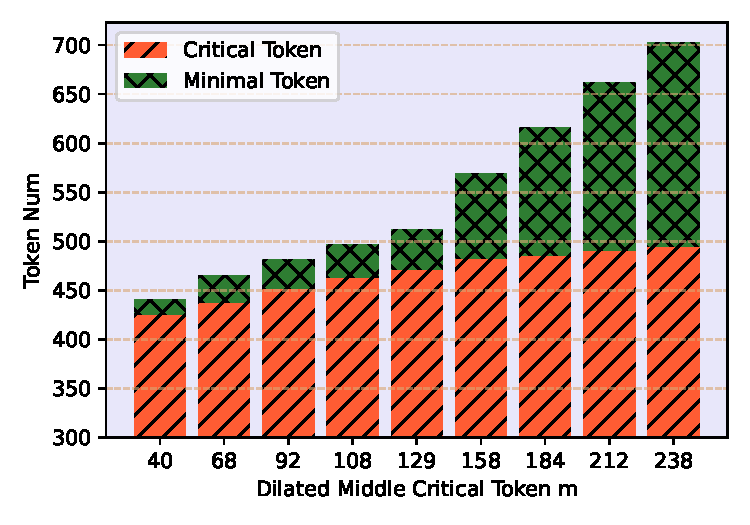
\includegraphics[width=0.4\textwidth]{assets/cis-dilation.pdf}
\centering
\vspace{-1em}
    \caption{\textbf{Effect of CIS dilation on LongBench NarrativeQA.} The stacked bar shows the average processed KV set: the \textcolor{orange}{orange segment} counts tokens that also appear in the top-$k$ oracle (budget 512, following Sec.~\ref{sec:longbench}), while the \textcolor{darkgreen}{green segment} counts minimal tokens not in the top-$k$ set.}
    \label{fig:cis-dilation}
    \vspace{-0.5em}
\end{figure}
%--------

%\paragraph{CIS Expansion}
\subsubsection{CIS Dilation}
\label{sec:cis-dilation}

We assess CIS dilation using the CIS$^\ast$ configurations from Sec.~\ref{sec:longbench}, varying the number of top indices dilated $m$. As shown in Fig.~\ref{fig:cis-dilation}, the number of \emph{additional} tokens beyond the top-$k$ set remains small for moderate $m$; dilation overhead grows gradually as $m$ increases, and the added tokens are predominantly low-importance. Inspecting shared queries explains this behavior as follows. Their most influential critical tokens are tightly clustered and spatially stable, so dilation contributes few extra indices. In contrast, when the budget begins to include low-score tokens, these indices are irregular and scattered, and dilation substantially inflates the set. This motivates restricting dilation to a top fraction of retrieved tokens. In practice, the expanded set also overlaps heavily with the remaining retrieved indices, further limiting redundancy.


\begin{table*}[t]
\centering
\caption{\textbf{Hyperparameter tuning on LLaMA2-Chat-7B for CPE.} The COQA setting for CIS follows the CIS$^\ast$ configuration, and HyperKV follows the HyperKV configuration, as described in Sec.~\ref{sec:gsm8k&coqa}. WikiText perplexity (PPL) is measured only during the prefilling stage. The Avg.Token measures the average processed tokens per head only in the decoding stage.}
\label{tab:hyper-tune}
\begin{tabular}{l|ccccccc|cccccc}
\toprule
Methods & $s$ & $\tau$ & $r$ & $\phi$ & $\psi$ & $\alpha$ & $\gamma$ & $\hat{\rho}$ & Avg. Token & Wiki PPL & GSM8K(flexible) & COQA(EM/F1)\\
\midrule
\multirow{4}{*}{CIS}
  & 4 & 0.8 & 1 & - & - & - & - & 0.301 & 124 & - & 0.1834 & 0.6023 / 0.7632\\
  & 8 & 0.7 & 1 & - & - & - & - & 0.152 & 131 & - & 0.1801 & 0.6090 / 0.7648\\
  & 8 & 0.8 & 2 & - & - & - & - & 0.184 & 167 & - & 0.1653 & 0.6083 / 0.7650\\
  & 32 & 0.8 & 1 & - & - & - & - & 0.0046 & 136 & - & 0.1693 & 0.6080 / 0.7641\\

\midrule

\multirow{2}{*}{PSAW}
  & - & - & - & 0.5 & - & 1 & - & - & - & 6.120 & 0.1896 & 0.5925 / 0.7568\\
  & - & - & - & 0.7 & - & 1.5 & - & - & - & 6.113 & 0.1803 & 0.5938 / 0.7573\\

\midrule

\multirow{2}{*}{ETF}
  & - & - & - & - & 0.5 & - & 1.5 & - & - & 6.162 & 0.1864 & 0.5962 / 0.7563\\
  & - & - & - & - & 0.4 & - & 1 & - & - & 6.156 & 0.1883 & 0.5962 / 0.7537\\

\midrule

\multirow{2}{*}{CPE}
  & 8 & 0.8 & 2 & 0.7 & 0.5 & 1.2 & 1.2 & 0.176 & 166 & 6.148 & 0.1348 & 0.5998 / 0.7591 \\
  & 32 & 0.8 & 1 & 0.7 & 0.5 & 1 & 1 & 0.0044 & 133 & 6.136 & 0.1634 & 0.5965 / 0.7572\\

\bottomrule
\end{tabular}
\end{table*}

%\paragraph{Ablation Studies}
\subsubsection{Hyperparameter Tuning}
\label{sec:hyper-tune}
\paragraph{Setting} We tune the key knobs of our compression pipeline in Table~\ref{tab:hyper-tune}. For \emph{CIS}, we adopt the CIS$^\ast$ configuration from Sec.~\ref{sec:gsm8k&coqa} and vary the block size $s$, similarity threshold $\tau$, and neighbor radius $r$. For \emph{PSAW} and \emph{ETF} in isolation, we apply them on dense attention, fix $\ell_s=\lfloor 3N/4\rfloor$, and control pruning/freezing aggressiveness via $(\phi,\alpha)$ for PSAW and $(\psi,\gamma)$ for ETF; PSAW is active in both prefill and decoding. For \emph{CPE}, we combine all three components, adding PSAW and ETF to CIS under TSA. We report: the averaged computation ratio $\hat{\rho}$, the average processed tokens per head in decoding (Avg.Token), \emph{prefill}-only WikiText perplexity (PPL), and task accuracy on GSM8K (flex) and COQA (EM/F1).

\paragraph{CIS} Varying $(s,\tau,r)$ reveals the accuracy–efficiency trade-off. Smaller $s$ increases retrieval frequency (higher $\hat{\rho}$), whereas enlarging to $s{=}32$ drives the retrieval ratio down to $\hat{\rho}{=}0.0046$ with only a modest GSM8K accuracy drop; COQA remains notably stable across all $s$. At fixed $s{=}8$, increasing the dilation radius to $r{=}2$ substantially enlarges the active set but yields negligible accuracy change on both GSM8K and COQA; inspection shows that the added neighbors often include low-importance tokens, perturbing the attention-mass distribution without benefits. Slightly loosening $\tau$ has little effect on accuracy. Overall, $s$ is the dominant lever for efficiency, while $\tau$ and $r$ offer fine-grained control of recall versus budget.

\paragraph{PSAW} Prefill pruning is gentle on language modeling quality and downstream accuracy. Increasing aggressiveness from $(\phi{=}0.5,\alpha{=}1)$ to $(\phi{=}0.7,\alpha{=}1.5)$ barely changes WikiText PPL, and COQA is essentially unchanged, while GSM8K (flexible match) decreases only slightly.

\paragraph{ETF} Freezing during prefill shows similarly small effects. Adjusting from $(\psi{=}0.5,\gamma{=}1.5)$ to $(\psi{=}0.4,\gamma{=}1)$ yields virtually identical PPL and a tiny trade between GSM8K and COQA. ETF is therefore a stable knob for further prefill savings and slightly milder freezing is a safe default setting.

\paragraph{CPE} Combining CIS with PSAW and ETF preserves efficiency while keeping quality competitive. With aggressive dilation ($r{=}2$), GSM8K dips to $0.1348$. Increasing block size and reducing dilation to $r{=}1$ lowers selection frequency and trims Avg. Token by ${\sim}20\%$, recovering GSM8K to $0.1634$ with COQA nearly unchanged. Overall, CPE performs best with moderate–large blocks, restricted dilation ($r{=}1$), and mild PSAW/ETF schedules.




%------------------------------------------------------------
\begin{table}[tb]
\centering
\footnotesize
%\normalsize
\caption{Variants of CIS on the similarity designs. The model is LlaMA2-7b-chat.}
\label{tab:cis_variant}
%\resizebox{\linewidth}{!}
{
\begin{tabular}{l|c|ccc}
\toprule
Method & $s$ & GSM8K (flexible/strict) & COQA\\ 
\midrule

%\multirow{2}{*}{Query} & 8  & 0.1744 / 0.1736 & 0.6093  \\ 
% & 16  & 0.1668 / 0.1653 & 0.6093 \\ 

% \midrule

\multirow{2}{*}{Key} & 8  & 0.1547 / 0.1482 & 0.5613 \\ 
 & 16  &  0.1405 / 0.1334 & 0.5608  \\ 

\midrule

\multirow{2}{*}{Hidden} &  8 & 0.1303 / 0.1289 & 0.5416  \\ 
 &  16 &  0.1121 / 0.1108 & 0.5214 \\ 

\bottomrule
\end{tabular}
}
\end{table}
%------------------------------------------------------------

%\paragraph{CIS Variant Designs}
\subsubsection{Similarity Ablations} 

We explore alternative similarity metrics for CIS derived from different representations. Concretely, we replace the default cosine similarity between \emph{query} embeddings (Eq.~\ref{eq:cos_sim}) with cosine similarity computed on (i) hidden states $\bx$ and (ii) key embeddings $\bk$, and evaluate under the CIS$^\ast$ configuration in Sec.~\ref{sec:gsm8k&coqa}. As shown in Table~\ref{tab:cis_variant}, both variants reduce accuracy, with the hidden-state metric degrading most. This indicates that the query, key, and hidden-state spaces emphasize distinct semantics; temporal semantic proximity for CIS is best captured in the \emph{query} space, whereas measuring similarity in $\bx$ or $\bk$ misaligns clusters and harms selection quality.
